\section{Giám sát và kiểm soát chi phí}
\label{sec:monitoring}

\subsection{CloudWatch Dashboard}
\label{ssec:cloudwatch_dashboard}

CloudWatch Dashboard cung cấp cái nhìn tổng quan về hoạt động của hệ thống thông qua các metrics quan trọng.

\subsubsection{Dashboard Configuration}

Dashboard được đặt tên "TaskManager-Dashboard" và bao gồm các widgets sau:

\begin{enumerate}
    \item \textbf{Lambda Invocations:} Hiển thị tổng số lần Lambda được gọi, giúp theo dõi traffic pattern.
    
    \item \textbf{Lambda Duration:} Hiển thị P50 và P99 percentile của thời gian thực thi Lambda, giúp phát hiện performance issues.
    
    \item \textbf{Lambda Errors:} Số lượng errors xảy ra trong Lambda function, quan trọng để phát hiện bugs.
    
    \item \textbf{Lambda Throttles:} Số lần Lambda bị throttle do vượt quá Reserved Concurrency limit.
    
    \item \textbf{API Gateway Latency:} End-to-end response time từ API Gateway, bao gồm cả Lambda execution time.
    
    \item \textbf{API Gateway 4XX/5XX Errors:} Client errors (4XX) và server errors (5XX) từ API Gateway.
\end{enumerate}

\begin{figure}[H]
\centering
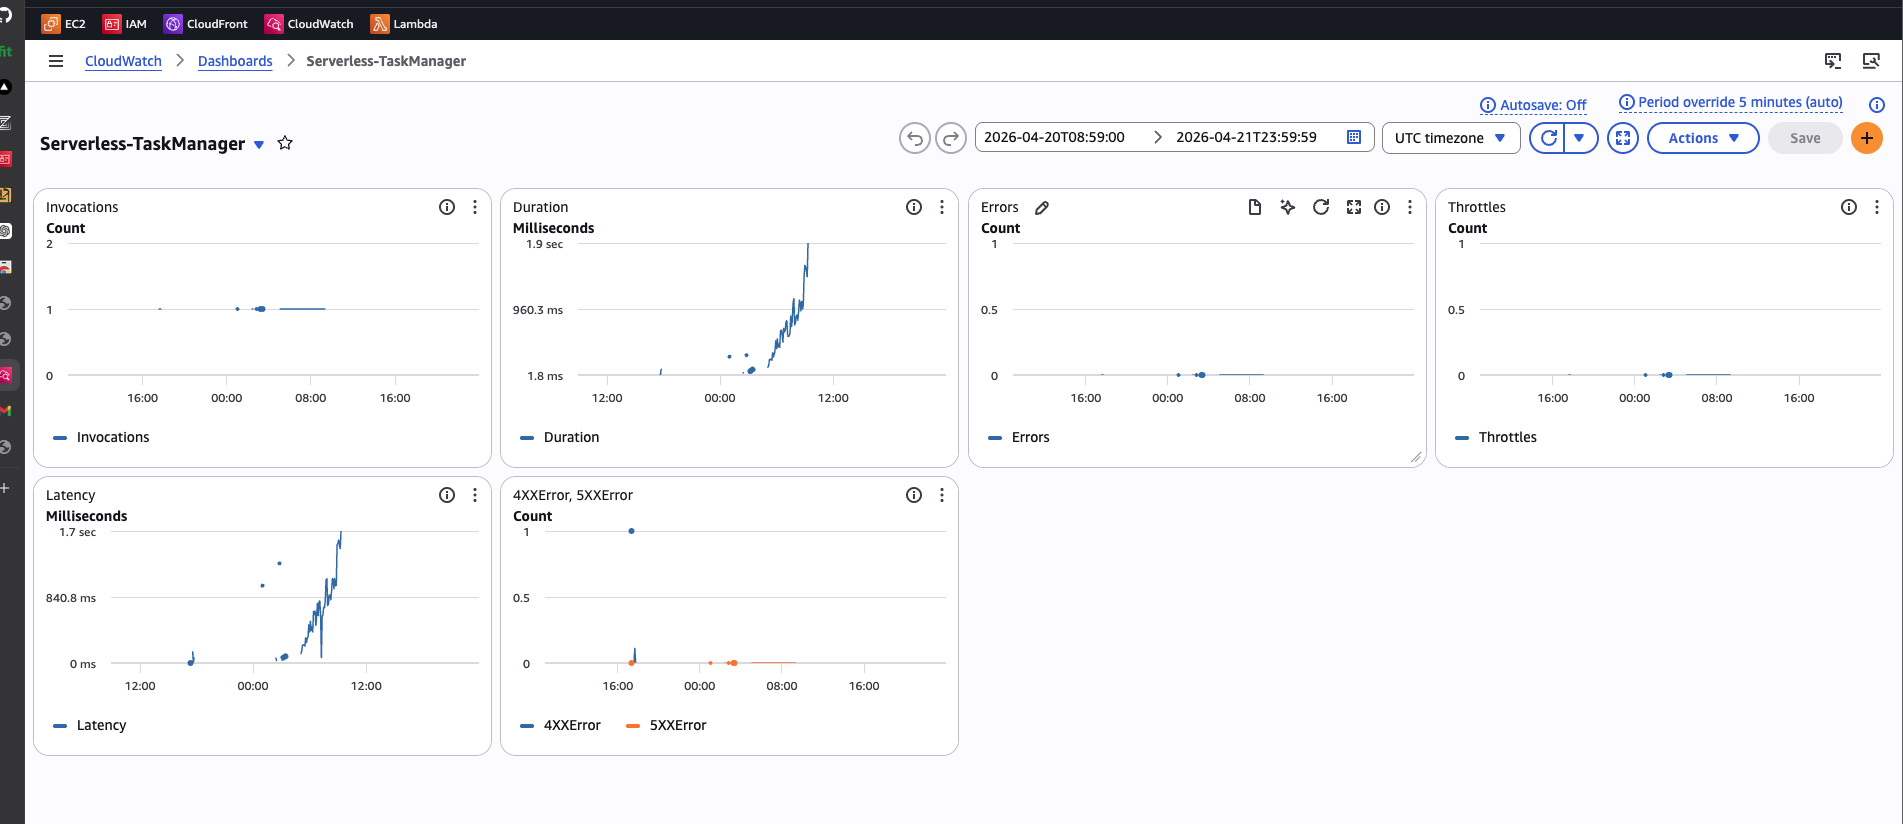
\includegraphics[width=\textwidth]{img/MON_cloudwatch_dashboard.png}
\caption{CloudWatch Dashboard với các metrics quan trọng}
\label{fig:cloudwatch_dashboard}
\end{figure}

Hình \ref{fig:cloudwatch_dashboard} cho thấy dashboard đang hoạt động với dữ liệu thực tế. Các metrics này giúp team:
\begin{itemize}
    \item Theo dõi performance và availability của hệ thống
    \item Phát hiện sớm các vấn đề tiềm ẩn
    \item Đánh giá impact của code changes
    \item Tối ưu hóa resource usage
\end{itemize}

\subsection{CloudWatch Alarms}
\label{ssec:cloudwatch_alarms}

Hệ thống được cấu hình với 2 alarms chính để phát hiện và thông báo khi có vấn đề xảy ra.

\subsubsection{Lambda Error Alarm}

\begin{itemize}
    \item \textbf{Alarm name:} Lambda-Error-Alarm
    \item \textbf{Metric:} AWS/Lambda - Errors
    \item \textbf{Condition:} Errors > 10 trong 5 phút
    \item \textbf{Action:} Gửi email qua SNS topic
    \item \textbf{Rationale:} Nếu có hơn 10 errors trong 5 phút, có thể có bug nghiêm trọng cần xử lý ngay
\end{itemize}

\subsubsection{API Gateway 5XX Alarm}

\begin{itemize}
    \item \textbf{Alarm name:} API-5xx-Alarm
    \item \textbf{Metric:} AWS/ApiGateway - 5XXError
    \item \textbf{Condition:} 5XXError > 5 trong 5 phút
    \item \textbf{Action:} Gửi email qua SNS topic
    \item \textbf{Rationale:} 5XX errors thường là server-side issues cần được xử lý ưu tiên cao
\end{itemize}

\begin{figure}[H]
\centering

\includegraphics[width=0.9\textwidth]{img/Alarm.png}
\caption{CloudWatch Alarms configuration}
\label{fig:alarms}
\end{figure}

Hình \ref{fig:alarms} hiển thị cả 2 alarms đã được cấu hình. Status có thể là:
\begin{itemize}
    \item \textbf{OK:} Metric nằm trong ngưỡng bình thường
    \item \textbf{ALARM:} Metric vượt ngưỡng, email notification được gửi
    \item \textbf{INSUFFICIENT\_DATA:} Chưa đủ dữ liệu để đánh giá
\end{itemize}

\subsubsection{SNS Email Notification}

Khi alarm được trigger, SNS gửi email notification đến team members.

\begin{figure}[H]
\centering

\includegraphics[width=0.9\textwidth]{img/Alarm-mail.png}
\caption{Email notification từ CloudWatch Alarm}
\label{fig:alarm_email}
\end{figure}

Hình \ref{fig:alarm_email} cho thấy email notification chứa:
\begin{itemize}
    \item Alarm name và description
    \item Metric details (namespace, metric name, dimensions)
    \item Threshold và actual value
    \item Timestamp khi alarm được trigger
    \item Link đến CloudWatch console để investigate
\end{itemize}

\subsection{CloudWatch Logs}
\label{ssec:cloudwatch_logs}

CloudWatch Logs tự động capture tất cả logs từ Lambda functions, giúp debugging và monitoring.

\subsubsection{Successful Request Log}

\begin{figure}[H]
\centering
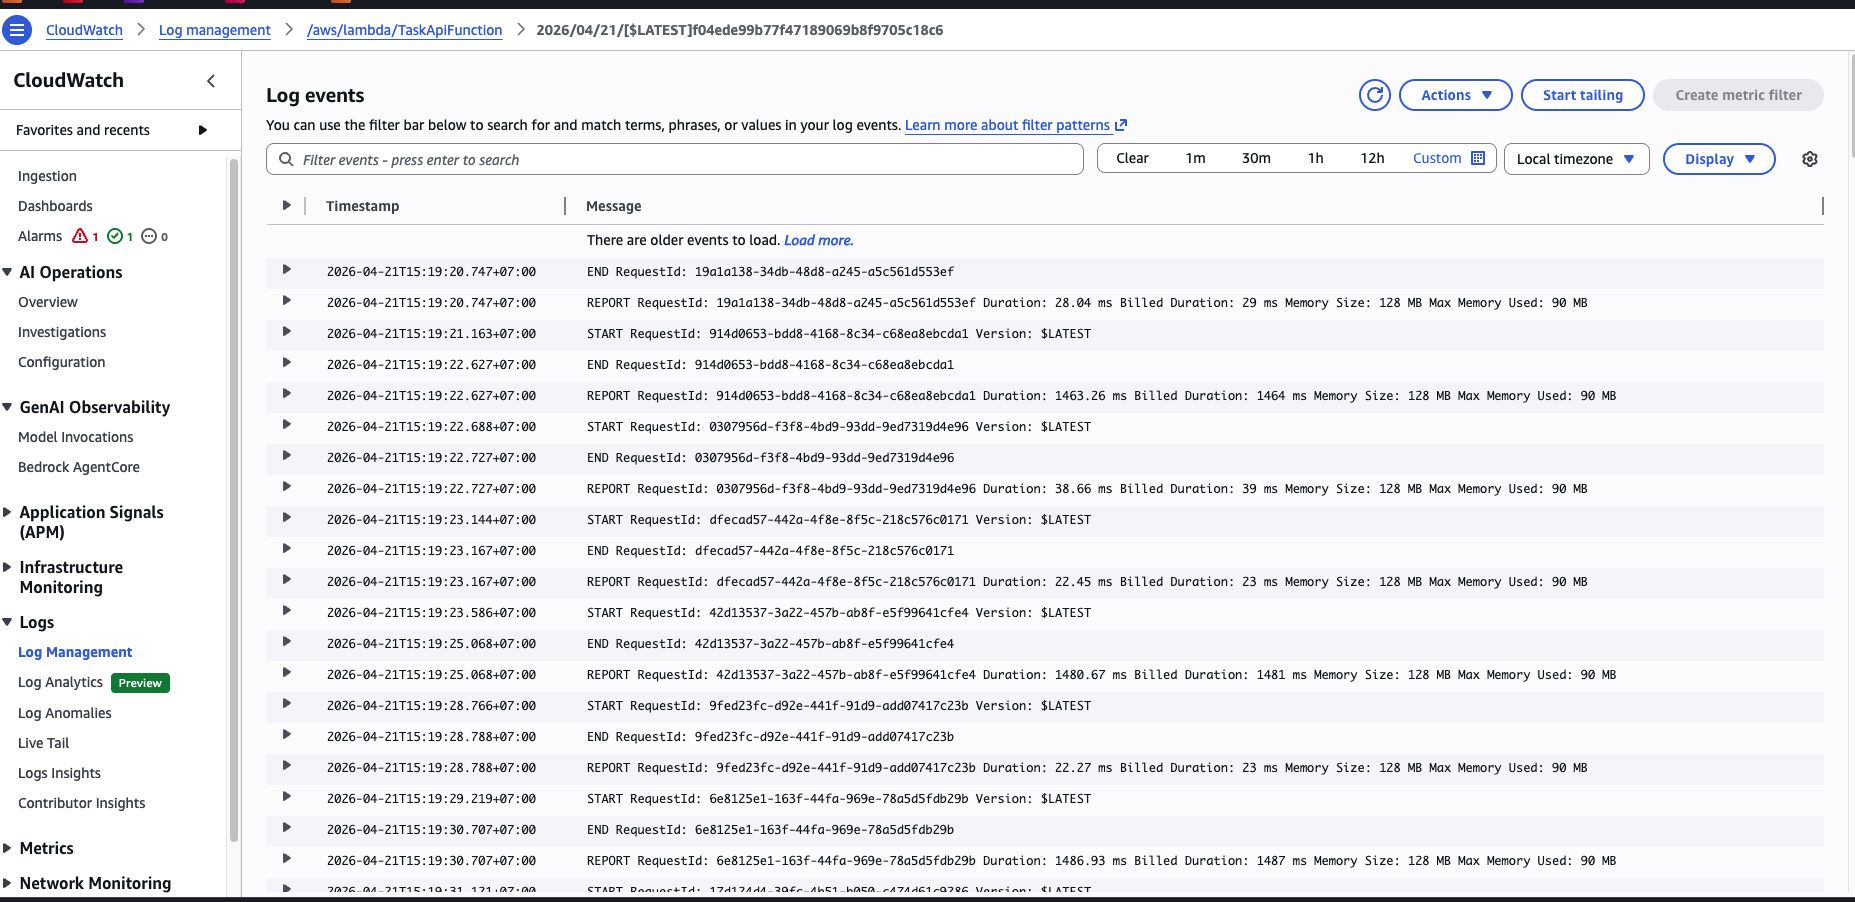
\includegraphics[width=\textwidth]{img/14-success-request.png}
\caption{CloudWatch log của successful request}
\label{fig:success_log}
\end{figure}

Hình \ref{fig:success_log} hiển thị log của một request thành công với:
\begin{itemize}
    \item \textbf{START:} Request ID và initialization
    \item \textbf{Application logs:} Custom logs từ Lambda code
    \item \textbf{REPORT:} Summary metrics
    \begin{itemize}
        \item Duration: Thời gian thực thi thực tế
        \item Billed Duration: Thời gian được tính phí (làm tròn lên 100ms)
        \item Memory Size: Memory được allocate
        \item Max Memory Used: Memory thực tế sử dụng
    \end{itemize}
\end{itemize}

\subsubsection{Error Request Log}

\begin{figure}[H]
\centering
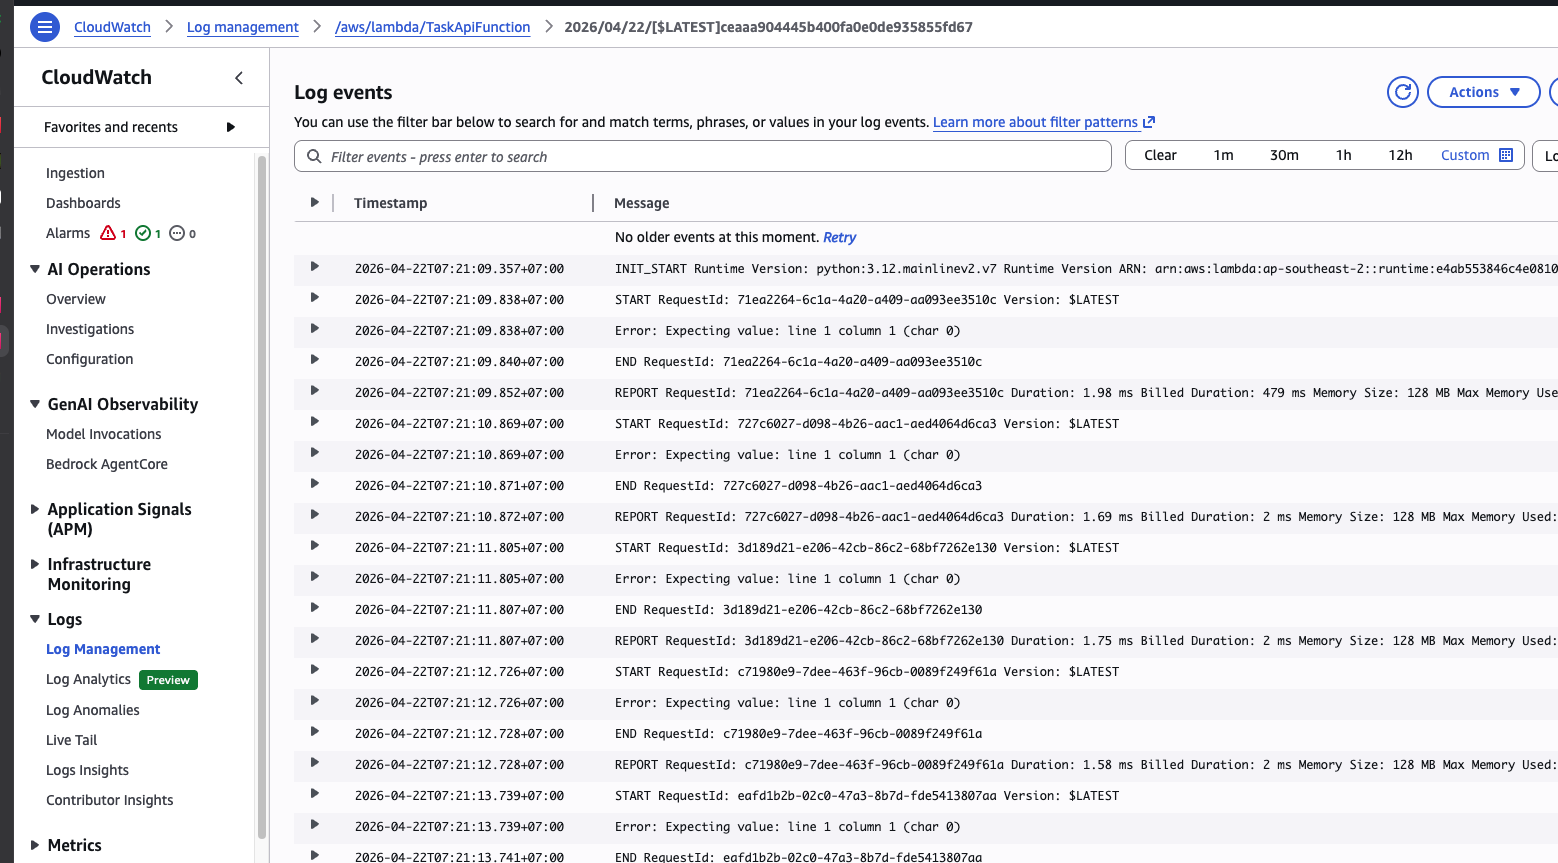
\includegraphics[width=\textwidth]{img/14-error-request.png}
\caption{CloudWatch log của error request}
\label{fig:error_log}
\end{figure}

Hình \ref{fig:error_log} cho thấy log khi có error xảy ra:
\begin{itemize}
    \item \textbf{ERROR:} Error message và stack trace
    \item \textbf{Exception details:} Type, message, và line number
    \item Giúp developers nhanh chóng identify và fix bugs
\end{itemize}

\subsection{AWS Budgets}
\label{ssec:aws_budgets}

AWS Budgets được cấu hình để kiểm soát chi phí và đảm bảo hệ thống không vượt quá Free Tier.

\subsubsection{Budget Configuration}

\begin{itemize}
    \item \textbf{Budget name:} TaskManager-Budget
    \item \textbf{Budget amount:} \$0.01 per month
    \item \textbf{Alert thresholds:}
    \begin{itemize}
        \item 80\% (\$0.008): Warning alert
        \item 100\% (\$0.01): Critical alert
    \end{itemize}
    \item \textbf{Notification:} Email qua SNS
\end{itemize}

\begin{figure}[H]
\centering
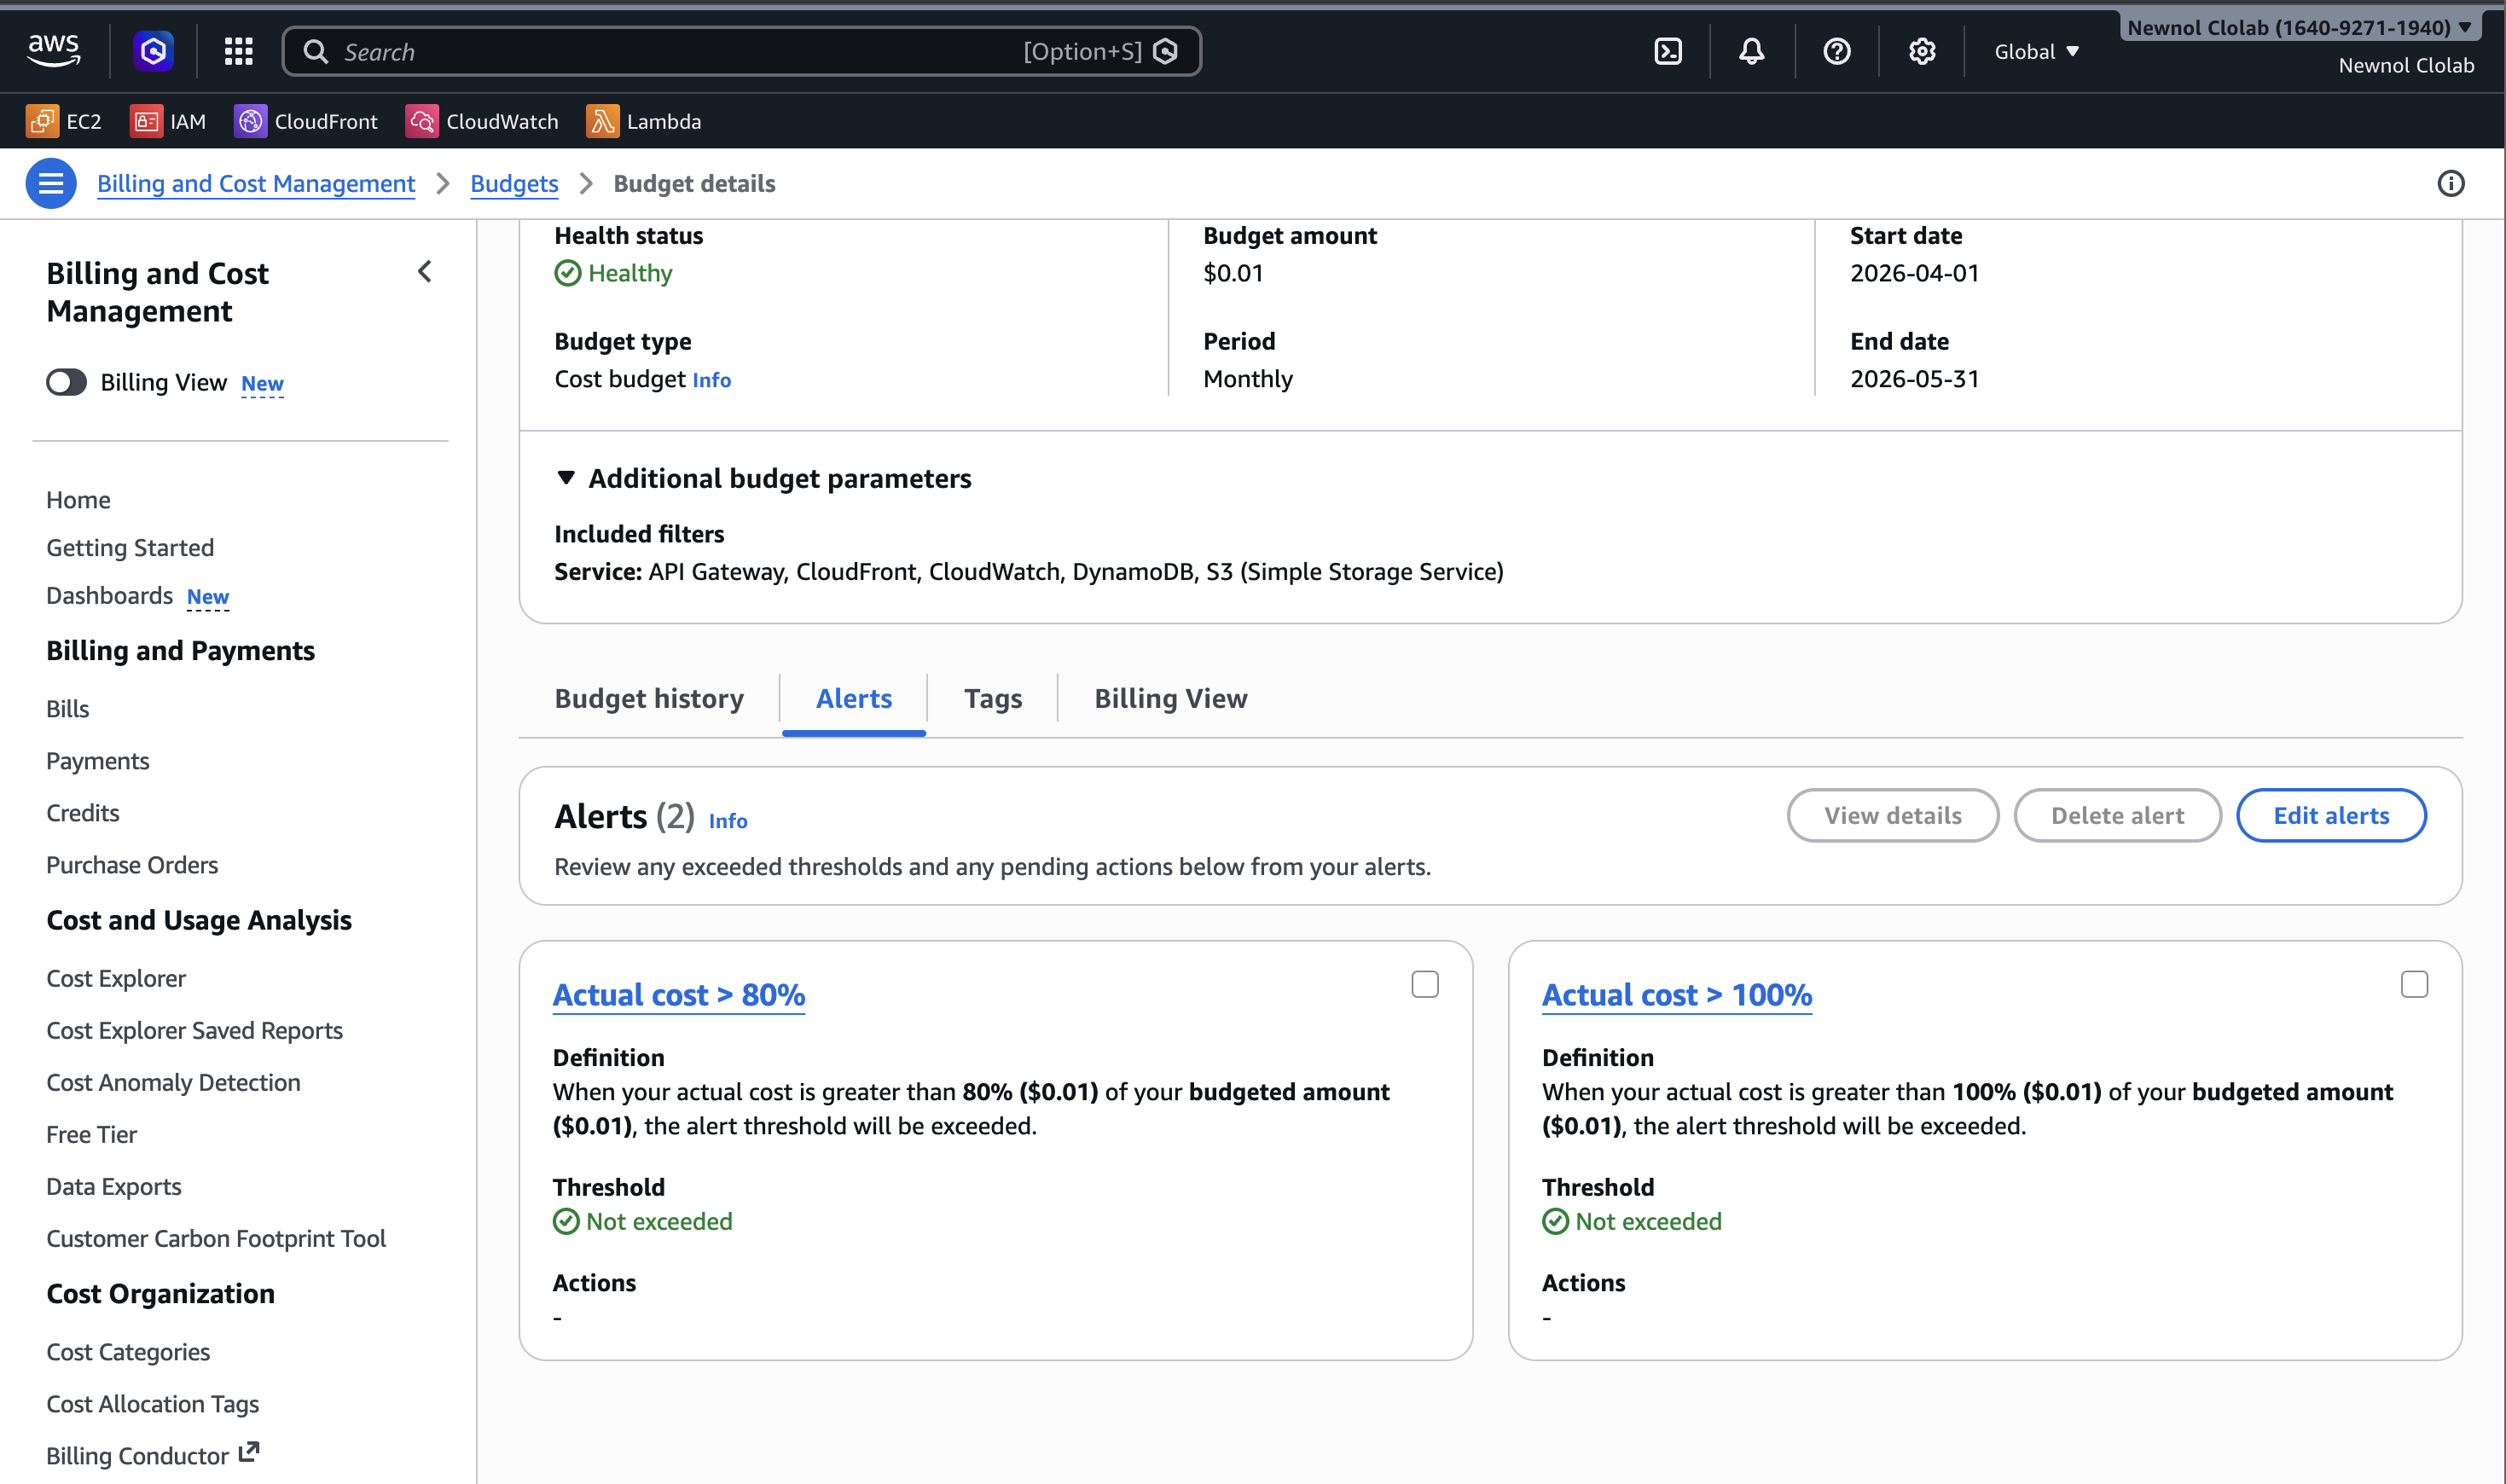
\includegraphics[width=\textwidth]{img/13-budget.png}
\caption{AWS Budgets configuration với \$0.01 limit}
\label{fig:budget}
\end{figure}

Hình \ref{fig:budget} hiển thị budget configuration. Khi chi phí đạt 80\% hoặc 100\%, email notification sẽ được gửi tự động.

\subsubsection{Budget Alert Email}

\begin{figure}[H]
\centering
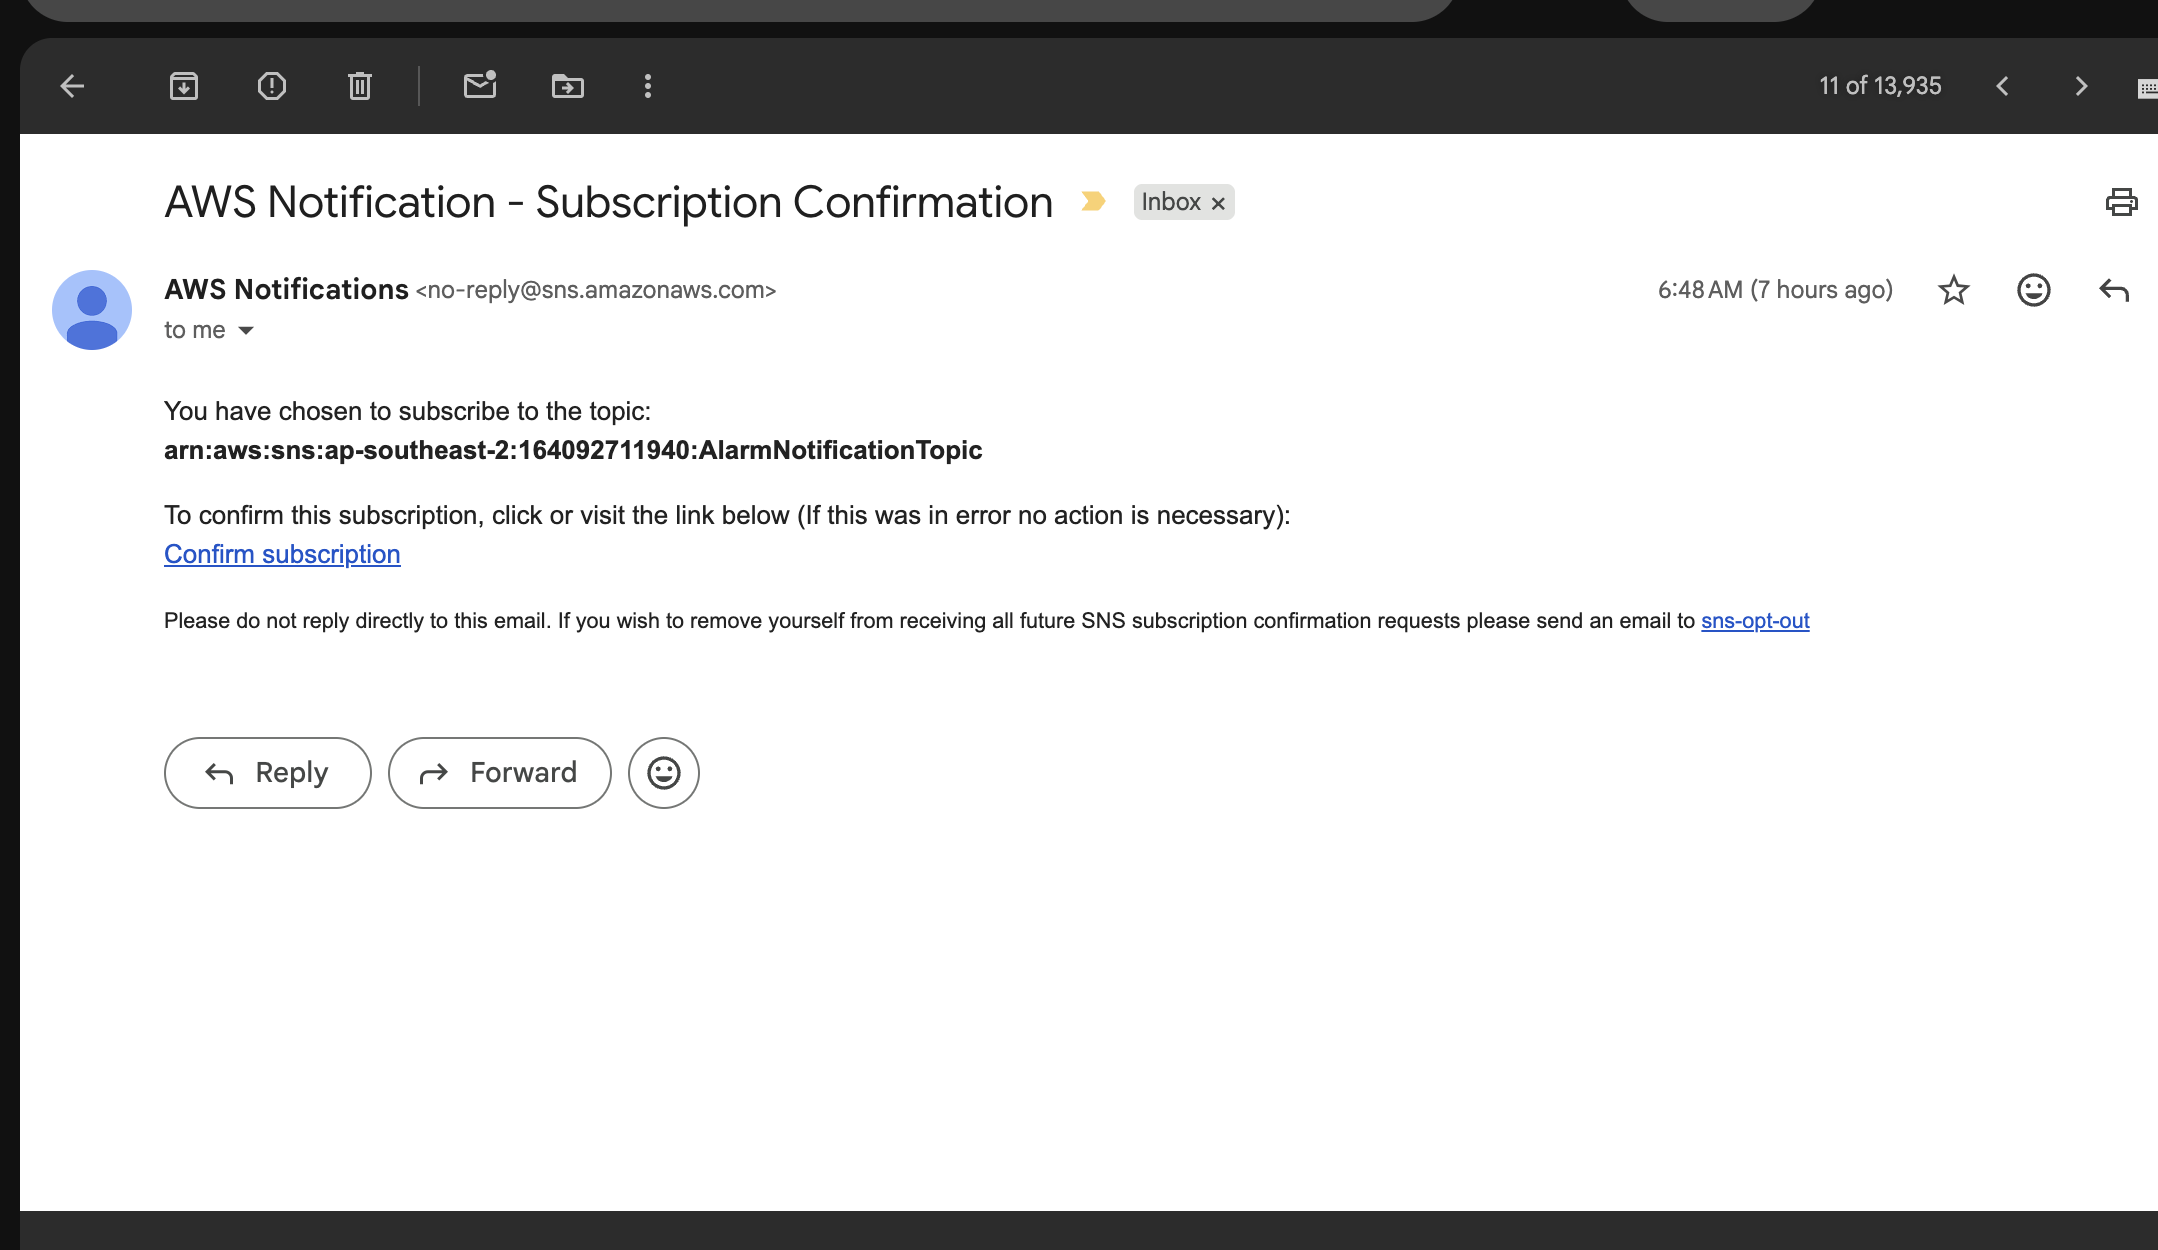
\includegraphics[width=0.9\textwidth]{img/13-email-confirm.png}
\caption{Email confirmation cho budget alerts}
\label{fig:budget_email}
\end{figure}

Hình \ref{fig:budget_email} cho thấy email subscription confirmation. Sau khi confirm, team sẽ nhận được alerts khi budget threshold được vượt qua.

\subsection{Cost Control Measures}
\label{ssec:cost_control}

Để đảm bảo chi phí bằng 0, các biện pháp sau đã được áp dụng:

\begin{table}[H]
\centering
\begin{tabular}{|l|p{6cm}|p{4cm}|}
\hline
\textbf{Service} & \textbf{Cost Control Measure} & \textbf{Free Tier Limit} \\
\hline
Lambda & Reserved Concurrency = 50 & 1M requests, 400K GB-seconds \\
\hline
API Gateway & Throttling: 100 req/s, burst 50 & 1M API calls \\
\hline
DynamoDB & On-Demand mode & 25 GB, 25 RCU/WCU \\
\hline
CloudFront & Cache optimization & 1 TB transfer, 10M requests \\
\hline
S3 & Minimal file size & 5 GB storage, 20K GET \\
\hline
VPC & No NAT Gateway, use VPC Endpoint & VPC Endpoint: Free \\
\hline
CloudWatch & Limited log retention & 5 GB logs, 10 custom metrics \\
\hline
\end{tabular}
\caption{Cost control measures cho từng service}
\label{tab:cost_control}
\end{table}

\subsection{Monitoring Best Practices}
\label{ssec:monitoring_best_practices}

Các best practices đã được áp dụng:

\begin{enumerate}
    \item \textbf{Structured Logging:} Lambda logs sử dụng JSON format để dễ dàng parse và analyze.
    
    \item \textbf{Correlation IDs:} Mỗi request có unique ID để trace qua các services.
    
    \item \textbf{Metric Dimensions:} Sử dụng dimensions để filter metrics theo function name, stage, etc.
    
    \item \textbf{Alert Fatigue Prevention:} Threshold được set hợp lý để tránh false positives.
    
    \item \textbf{Dashboard Organization:} Metrics được nhóm theo layer (API, Compute, Database).
    
    \item \textbf{Cost Monitoring:} Daily check AWS Cost Explorer để phát hiện sớm unexpected charges.
\end{enumerate}

\subsection{Tổng kết Monitoring}
\label{ssec:monitoring_summary}

Hệ thống monitoring đã được triển khai đầy đủ với:

\begin{itemize}
    \item ✓ CloudWatch Dashboard với 6+ widgets hiển thị real-time metrics
    \item ✓ 2 CloudWatch Alarms với SNS email notifications
    \item ✓ CloudWatch Logs capturing successful và error requests
    \item ✓ AWS Budgets với \$0.01 limit và 2 alert thresholds
    \item ✓ Cost control measures đảm bảo chi phí = \$0
\end{itemize}

Hệ thống monitoring này cung cấp full observability và cost control, đáp ứng đầy đủ yêu cầu của đề tài.
